\documentclass[letterpaper,10 pt,conference]{ieeeconf}

\IEEEoverridecommandlockouts
\overrideIEEEmargins
\bibliographystyle{IEEEtran}

\usepackage{graphics,epsfig,mathptmx,times,amsmath,amssymb,graphicx,booktabs}
\usepackage[lite,subscriptcorrection,slantedGreek,nofontinfo]{mtpro2}
\usepackage[ruled,vlined]{algorithm2e}
\usepackage[english]{babel}
\usepackage{blindtext}

\input defs.tex

\title{\LARGE \bf
Player Behavior and Optimal Team Composition in\\
Online Multiplayer Games
}

\author{Hao Yi Ong$^{1}$, 
        Sunil Deolalikar$^{2}$ and 
        Mark V. Peng$^{3}$%
\thanks{$^{1}$Mechanical Engineering Department, 
        Stanford University}%
\thanks{$^{2}$Aeronautics and Astronautics Department, 
        Stanford University}%
\thanks{$^{3}$Computer Science Department, 
        Stanford University}%
\thanks{Email: {\tt\small $\{$haoyi,sunild93,mvpeng$\}$@stanford.edu}}
}

\begin{document}

\maketitle
\thispagestyle{plain}
\pagestyle{plain}

\begin{abstract} % under 150 words

We consider clustering player behavior and learning the optimal team composition for multiplayer online games. The goal is to determine a set of descriptive play style groupings and learn a predictor for win/loss outcomes. The predictor takes in as input the play styles of the participants in each team; i.e., the various team compositions in a game. Our framework uses unsupervised learning to find behavior clusters, which are, in turn, used with classification algorithms to learn the outcome predictor. For our numerical experiments, we consider League of Legends, a popular team-based role-playing game developed by Riot Games. We observe the learned clusters to not only corroborate well with game knowledge, but also provide insights surprising to expert players. We also demonstrate that game outcomes can be predicted with fairly high accuracy given team composition-based features.

\end{abstract}

\begin{keywords}

team performance, team composition, player behavior, video games, multiplayer games, game prediction

\end{keywords}

\section{Introduction}

Online virtual worlds are an increasingly significant venue for human interaction. By far the most active virtual worlds belong to a genre of video games called massively multiplayer online role-playing games (MMORPGs), where players interact with each other in a virtual world \cite{TSF:13}. In an MMORPG, players assume the role of in-game characters and take control over most of their characters' actions, often working in teams to accomplish a common objective, such as defeating opposing teams. Due to the shared, persistent nature of these virtual worlds, user behaviors and experiences are shaped by various social factors. 

Besides profit-making, an understanding of these social dynamics would provide insight to human interactions in the real world and the potential of virtual worlds for education, training, and scientific research \cite{Bai:12,Dic:05}. Numerous prior studies in social sciences and management have investigated how team compositions can affect team performance \cite{Spo:11,HA:08}. However, little is understood about player behavior and team performance and factors contributing to it in competitive MMORPGs. To address this, we develop a machine learning framework that uses game histories to learn player behavior clusters and predict the outcome of games given prior knowledge about the game and its players. 

The contributions of this paper are twofold. First, we present several approaches that group player behaviors in online games. Second, we develop predictors that determine how likely it is that a team of players can emerge victorious given the said team's composition of players, all of whom may have different play styles. Specifically, we consider k-means and DP-means---an expectation maximization algorithm \cite{KJ:12}---for clustering play styles and logistic regression, Gaussian discriminant analysis, and support vector machines for determining win/loss outcomes. The rest of the paper is structured as follows. Section~II describes the target game of our numerical experiments and our data collection method. Sections~III and IV demonstrate several methods and their effectiveness for learning play style clusters and outcome predictors. Some concluding remarks are drawn and future works mentioned in Section~V.

\section{Target Game Description}

We begin with a description of the MMORPG used for our numerical experiments and the data acquisition method.

\subsection{League of Legends}

For this project we consider a popular MMORPG---the League of Legends (LoL). LoL is a multiplayer online battle arena video game developed and published by Riot Games with 27 million daily players \cite{Tas:14}. In this MMORPG, a standard game consists of two opposing teams of five players. Each player assumes the role of one of over 120 different characters battling each other to destroy the opposing team's ``towers''---structures that fall after suffering enough attacks from characters. A game is won when all of either team's towers are destroyed. 

\subsection{Data set acquisition}

The developer of LoL has made the game's player statistics and match histories freely available through a web-based application programming interface (API) \cite{Rio:14}. We randomly gathered over 100,000 instances of player statistics and over 10,000 instances of match histories from the 2013-2014 season. We then parsed and cleaned the raw game data to construct our training and testing sets, depending on the features we chose. Player statistics include performance indicators such as average damage dealt and number of wins. Match histories contain information such as participant ID numbers and character choices.

\section{Behavioral Clustering}

The target game's developers have grouped the 120 different in-game characters into six classes, such as assassin or support, which indicates the character's gameplay style. While these classes reflect the developers' design intent for the characters, they do not necessarily reveal the behavior of actual players in games. Using statistics from various players, we present our feature selection method and the gameplay styles learned by applying various clustering algorithms to our data set. We validate our results and the insights derived from it with expert analysis from ranked players.

\subsection{Feature selection}

For our clustering algorithms, the features were 21 normalized player statistics, such as average damage dealt and money earned. The statistics were normalized over their range of values, preventing clusters from being formed due to order of magnitude differences between statistics. For instance, damage dealt values are often 7 orders of magnitude greater than kill streaks, which means small variations in damage dealt are erroneously considered as much more important than kill streaks if taken directly as feature values. 

\subsection{Clustering algorithms}

\subsubsection{k-means}

Given a set of observations, k-means clustering aims to partition them into k sets $\mathcal{S} = \left\{ S_{1},\ldots,S_{k} \right\}$ so as to minimize the within-cluster sum of squares; i.e., find the minimizer $\mathcal{S}^{\star}$ of the distortion function:
\begin{align}
  \sum_{i=1}^{k}\sum_{x \in S_{i}}\left\| x - \mu_{i} \right\|_{2}^{2},
  \label{eqn:k-means}
\end{align}
where $x$ is an observation and $\mu_{i}$ is the $i^{th}$ cluster centroid.

In general, this problem is computationally difficult (NP-hard). For our clustering, we employ Lloyd's algorithm, which is a heuristic that consists of randomly choosing observations as cluster centroids and iteratively assigning observations to their closest centroids and updating the centroids with the mean of their respective clusters \cite{Ng:14}. 

To select the number of clusters $k$, we run 10-fold cross validation over $k$ to find a local optimizer. The scoring function for the cross validation is simply the average distortion given by \eqref{eqn:k-means} over the held-out sets. 

\subsubsection{DP-means}

DP-means is a nonparametric expectation-maximization (EM) algorithm derived using a Dirichlet process (DP) mixture of Gaussians model. In other words, the user does not choose the number of clusters beforehand. The technique being the topic of a series of papers, we will only provide a brief description of the algorithm. The reader is referred to \cite{TKJ:13,KJ:12} for a thorough review of DP-means. 

The derivation of DP-means is inspired by the connection between k-means EM with a finite mixture of Gaussians model. Namely, the k-means algorithm may be viewed as a limit of the EM algorithm if all of the covariance matrices corresponding to the clusters in a Gaussian mixture model are equal to $\sigma I$. As $\sigma \rightarrow 0$, the negative log-likelihood of the mixture of Gaussians model approaches the k-means clustering objective \eqref{eqn:k-means}. Correspondingly, the EM steps approach the k-means steps in Lloyd's algorithm. 

In the case of DP-means, \cite{KJ:12} shows how to perform a similar limiting argument. Specifically, if the generative model for the EM algorithm was a DP mixture of Gaussians model with $\sigma I$, letting $\sigma \rightarrow 0$ yields the objective function
\begin{align}
  \sum_{i = 1}^{k}\sum_{x \in S_{i}} \left\| x - \mu_{i} \right\|_{2}^{2} + \left(k - 1\right)\lambda^{2},
  \label{eqn:dp-means}
\end{align}
where $\mathcal{S} = \left\{ S_{1},\ldots,S_{k} \right\}$ is the set of clusters, $x$ is an observation, and $\mu_{i}$ is the $i^{th}$ cluster centroid. Note that, unlike in k-means, $k$ is now a variable to be optimized over.

This leads to an algorithm with clustering assignments similar to the classical k-means algorithm and the same monotonic local convergence guarantees. (See Algorithm~\ref{alg:dp-means}.) The difference is that a new cluster is formed whenever an observation is sufficiently far away from all existing cluster centroids, with some user-defined threshold distance $\lambda$. Intuitively, $\lambda$ is a penalty on the number of clusters, on top of the original k-means distortion function. 

\begin{algorithm}[!htbp]
  \caption{DP-means}

  \DontPrintSemicolon

  \SetKwInOut{Input}{input}
  \SetKwInOut{Output}{output}
  
  \Input{$\mathcal{X}$: input data, $\lambda$: threshold distance}
  \Output{Clustering $S_{1},\ldots,S_{k}$, number of clusters $k$}
  
  \smallskip

  $k \leftarrow 1$ \\
  $S_{1} \leftarrow$ random observation $\left\{x^{\text{rand}}\in\mathcal{X}\right\}$ \\
  $\mu_{1} \leftarrow x^{\text{rand}}$

  \Repeat{
    % termination condition
    $S_{1},\ldots,S_{k}$ converge
  }{
    % loop
    $X^{\text{perm}} \leftarrow$ random ordered permutation of $\mathcal{X}$ \\
    // cluster assignments \\
    \For{
      % iteration condition
      $x \in X^{\text{perm}}$ in order
    }{
      % loop
      $c \leftarrow \argmin_{i \in \left\{1,\ldots,k\right\}} \left\| x - \mu_{i} \right\|_{2}^{2}$ \\
      \If{
        % if condition
        $\left\| x - \mu_{c} \right\|_{2}^{2} > \lambda^{2}$
      }{
        % operation
        $k \leftarrow k + 1$ \\ 
        $\mu_{k} \leftarrow x$
      }
      \Else{
        % operation
        $\mathcal{S}_{c} \leftarrow \mathcal{S}_{c} \cup \left\{ x \right\}$
      }
    }
    // centroid updates \\
    \For{
      % iteration condition
      $i = 1,\ldots,k$
    }{
      % loop
      $\mu_{i} \leftarrow \frac{1}{\left|S_{i}\right|} \sum_{x \in S_{i}} x$
    }
  }

  \label{alg:dp-means}
\end{algorithm}

We ran DP-means with 10-fold cross validation over a range of $\lambda$ values, setting our scoring function as the average of the objective values from \eqref{eqn:dp-means} over the held-out sets.

\subsection{Results and interpretation}



\begin{figure}[htbp!]
  \centering
  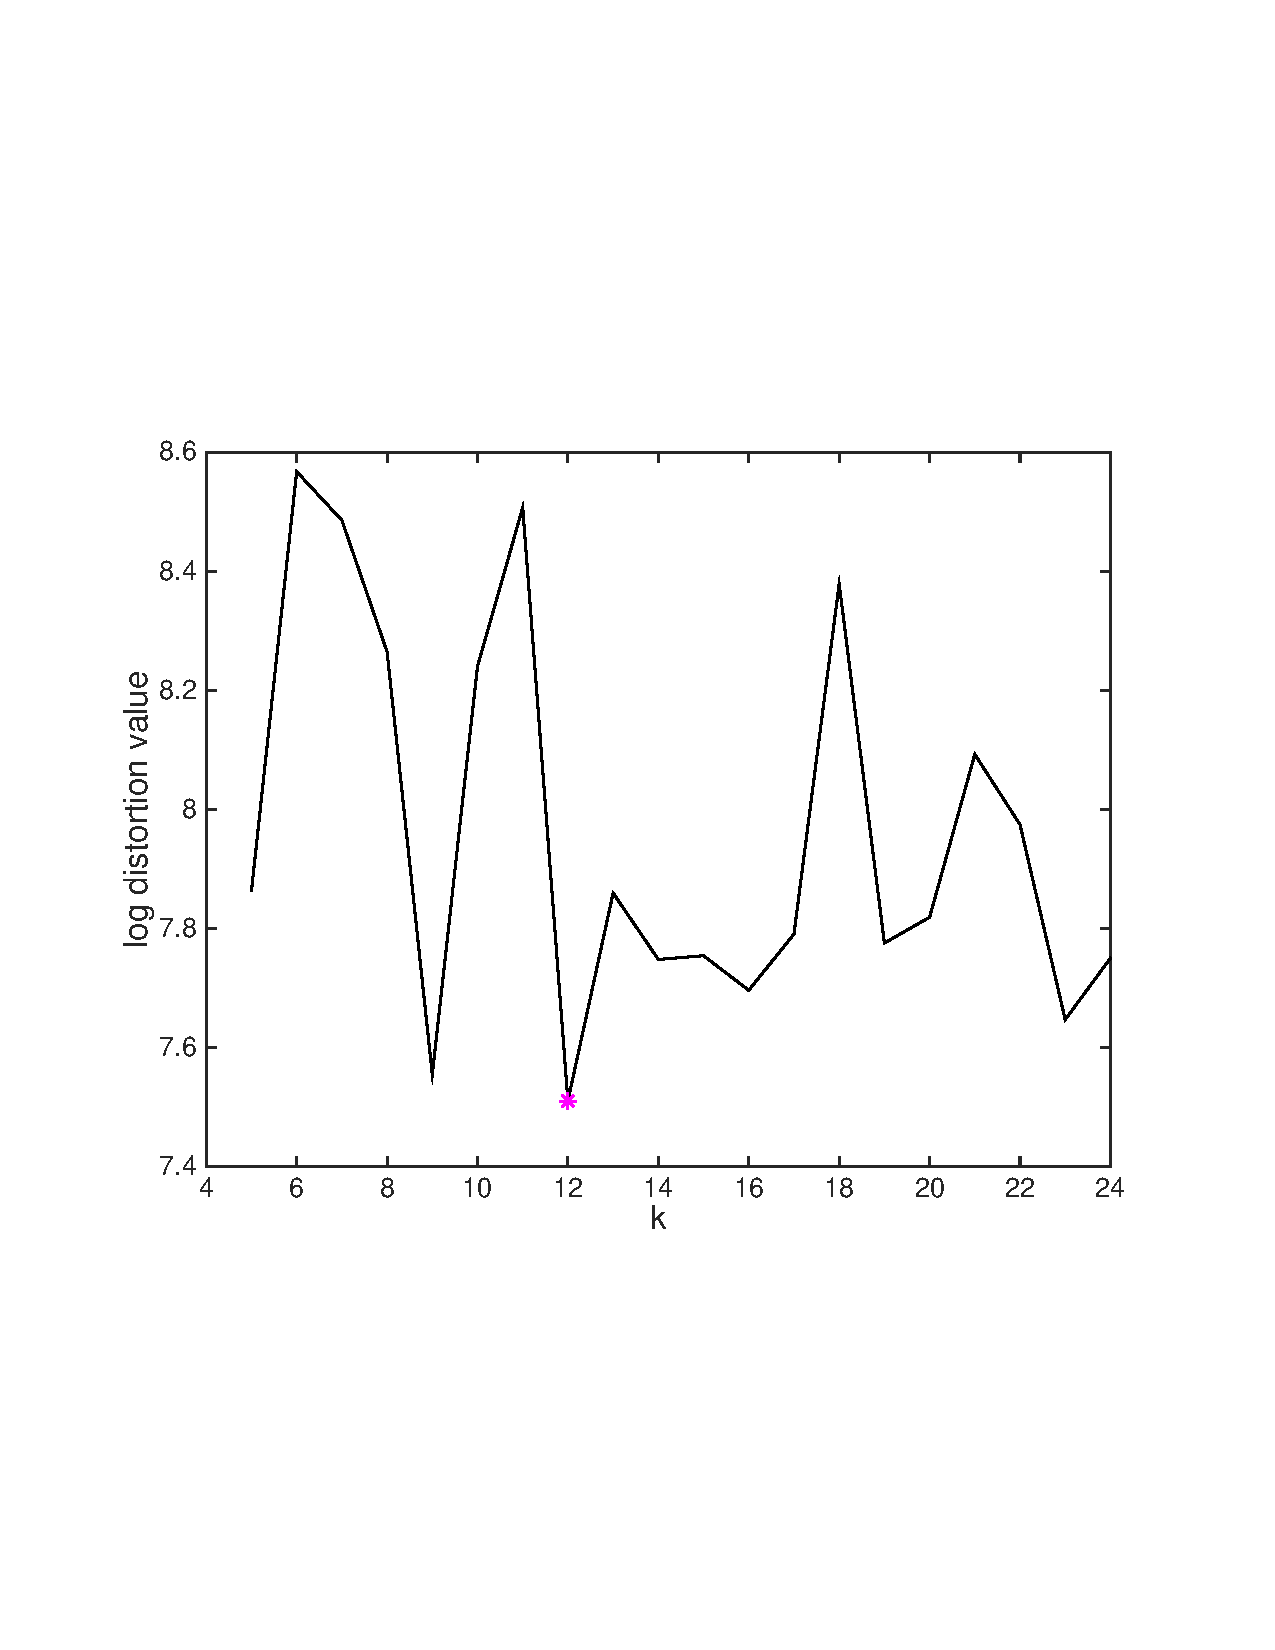
\includegraphics[trim=55pt 200pt 70pt 200pt, clip, width=0.48\textwidth]{km-conv.pdf}
  \caption{The log distortion values show a local optimum at k = 12 over the range of 5 to 24 clusters (highlighted above as a magenta asterisk).}
  \label{fig:kmeans-conv}
\end{figure}

\begin{table}[htbp!]
  \centering
  \caption{Play style clustering summary results}
  \begin{tabular}{lcccc}
    \toprule
    & cross validation & no. of clusters & cpu time \\ \midrule
    k-means & 10-fold & 12 & 154.1 s \\
    DP-means & 10-fold & 8 & 65.4 s \\
    \bottomrule
  \end{tabular}
  \label{tab:clus}
\end{table}

\subsection{Cluster visualization with PCA}

Fig.~\ref{fig:viz} shows the result of applying principal component analysis (PCA) to reduce our feature dimension and visualize it in three dimensions. Notice that the data is clearly clustered into 8 distinct groups, suggesting that in higher dimensions there are probably more clusters. Overlaying our 12-groups clustering from the k-means technique in color, we observe that they are consistent with the PCA results: Almost all points in any k-means cluster are in the same PCA cluster. 

\begin{figure}[htbp!]
  \centering
  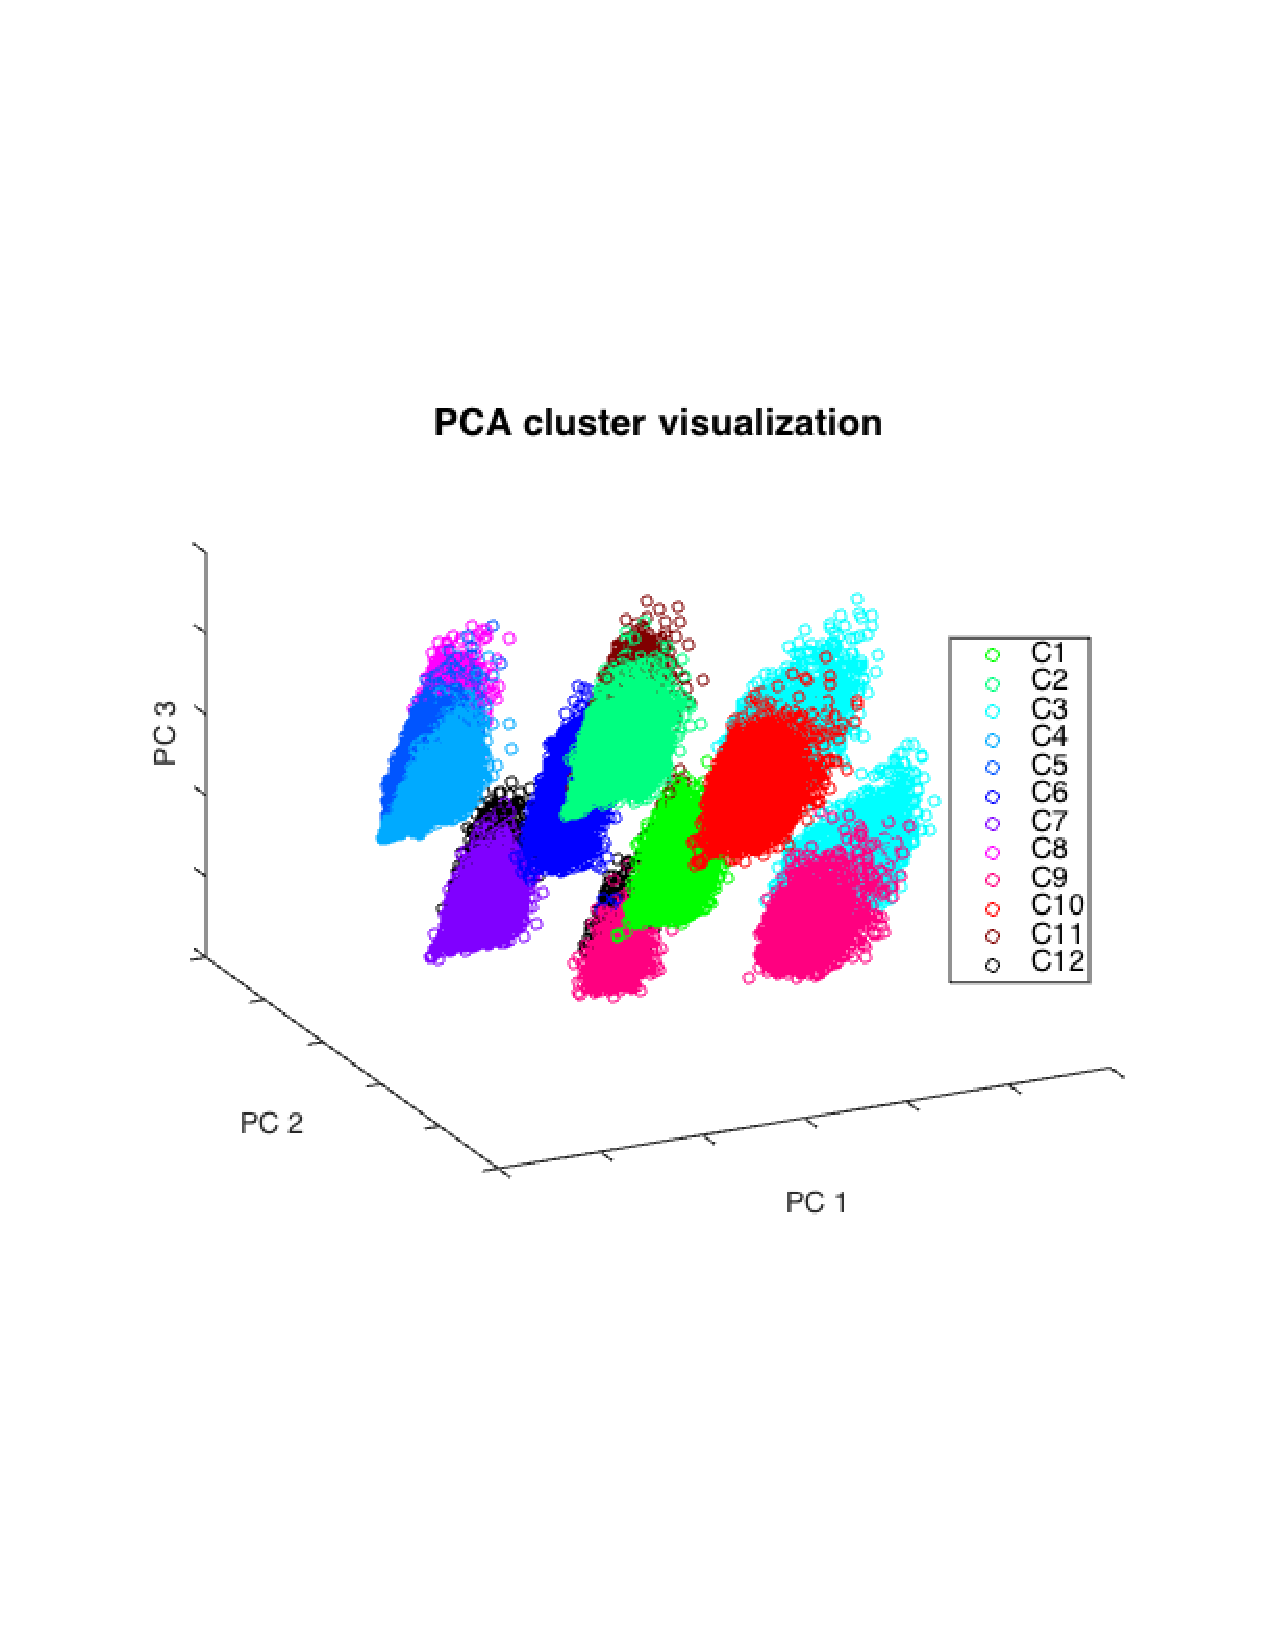
\includegraphics[trim=70pt 210pt 70pt 250pt, clip, width=0.48\textwidth]{viz-cluster.pdf}
  \caption{Visualizing our data with 3 principal components reveals at least 8 distinct clusters. The 12-clusters k-means results are overlaid in color.}
  \label{fig:viz}
\end{figure}

\section{Game Outcome Prediction}



\subsection{Feature selection}

For our classification algorithms, the features are the two teams' player compositions. Associated with each team is a vector of counts of players that fall into a certain play style category, which were, say, derived from one of the clustering algorithms. The feature vector is the concatenation of the count vectors of teams 1 and 2. The labels for each sample are the win/loss indicator for the game, with 1 corresponding to a victory and 0 a loss by team 1 to team 2. For instance, there are 8 clusters, teams 1 and 2 have the count vectors $x_{1}\in\reals^{8}$ and $x_{2}\in\reals^{8}$, and team 1 beats team 2. The feature vector-label pair would then be 
\[
  \left(x, y\right) = 
  \left(
    \left[
      \begin{array}{c}
        x_{1} \\ 
        x_{2}
      \end{array}
    \right],
    1
  \right).
\]

\subsection{Baseline evaluation criteria}



\subsection{Classification algorithms}

\subsubsection{Logistic regression}



\subsubsection{Gaussian discriminant analysis}



\subsubsection{Support vector machine}



\subsection{Results and discussion}



\begin{table}[htbp!]
  \centering
  \caption{Outcome prediction summary results}
  \begin{tabular}{lcccccc}
    \toprule
    & \multicolumn{3}{c}{k-means} & \multicolumn{3}{c}{DP-means} \\
    & train acc. & test acc. & cpu time & train acc. & test acc. & cpu time \\ \midrule
    LR & 72.25\% & 68.75\% & 7.4 s & 69.67\% & 67.11\% & 7.1 s \\
    GDA & 74.79\% & 70.14\% & 7.7 s & 70.88\% & 68.39\% & 7.1 s \\
    SVM & 74.75\% & 70.39\% & 91.2 s & 71.71\% & 69.21\% & 41.6 s \\
    \bottomrule
  \end{tabular}
  \label{tab:pred}
\end{table}

\section{Conclusion and Extensions}



\section*{Acknowledgments}
The authors thank Prof. Andrew Ng and the course staff.

\bibliography{IEEEabrv,report}

\end{document}